\chapter{Aspartate in cellular metabolism}
blaa

\section{Introduction}
More blaa

\subsection{Intro subject 1}
qwerty

\subsection{Intro subject 2}
qwerty
\subsection{Details}
qwerty1


\begin{figure}
    \centering
    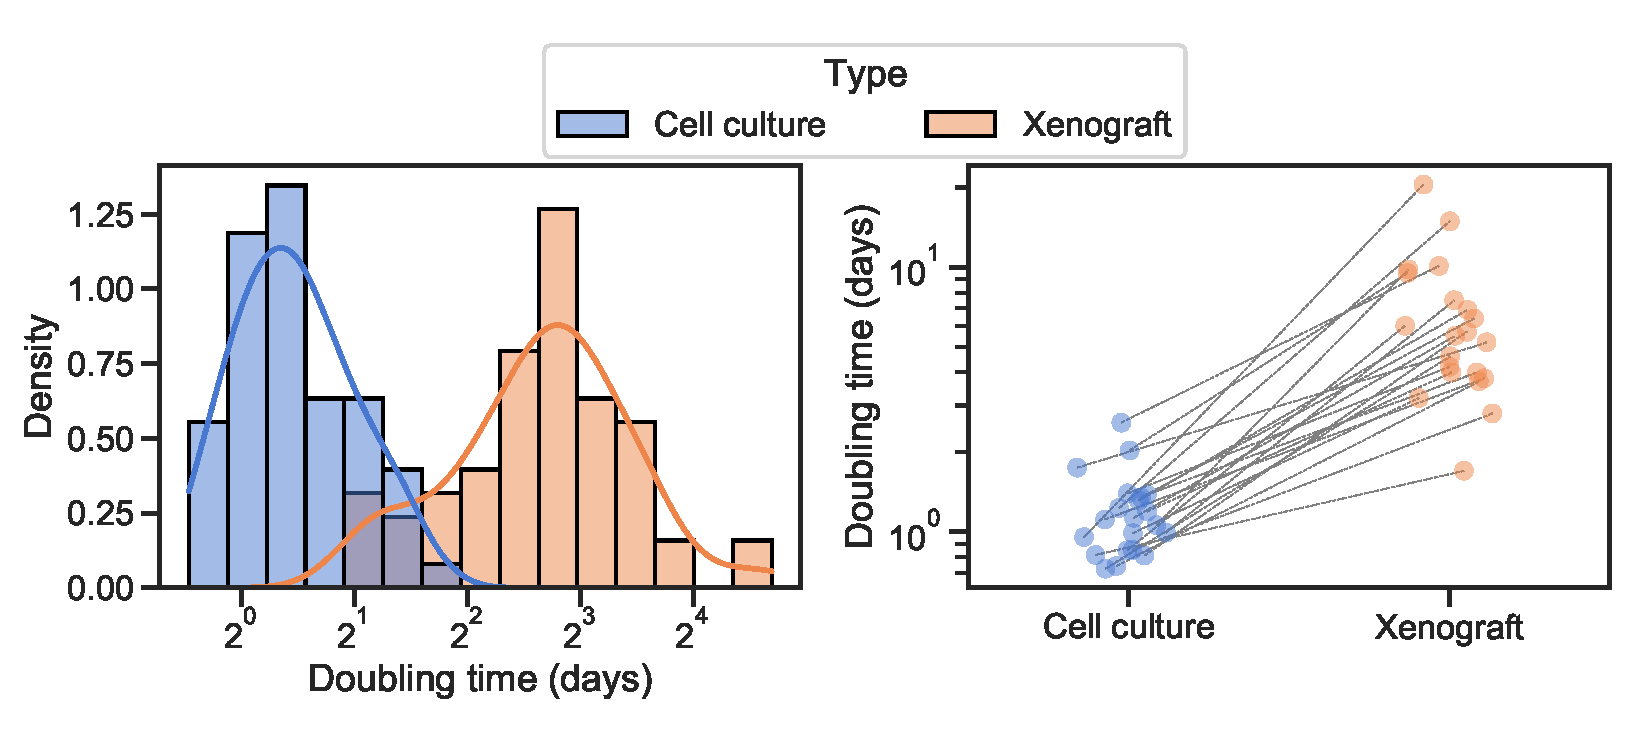
\includegraphics[width=0.70\textwidth]{figures/chap1/prlfr_contr.pdf}
    \caption[gggg]{
    gggg
    }
    \label{fig:ch1:prlfr_contr}
\end{figure}










Aspartate is typically coupled to NAD+/NADH ratio and thus if one is changed the other one is changed proportionally an vice versa.
Therefore it could be compelling to think that aspartate levels correlate with proliferation only indirectly through the NAD+/NADH ratio.
However, we have evidence against this:
Lucas' previous papers
My NAD+/NADH experiment with 143B SLC1A3 cells
Maddie's paper on SHDB which shows the opposite trend i.e. increased cytoplasmic NAD+/NADH ratio (due to media pyruvate) but are still aspartate limited



\begin{figure}
    \centering
    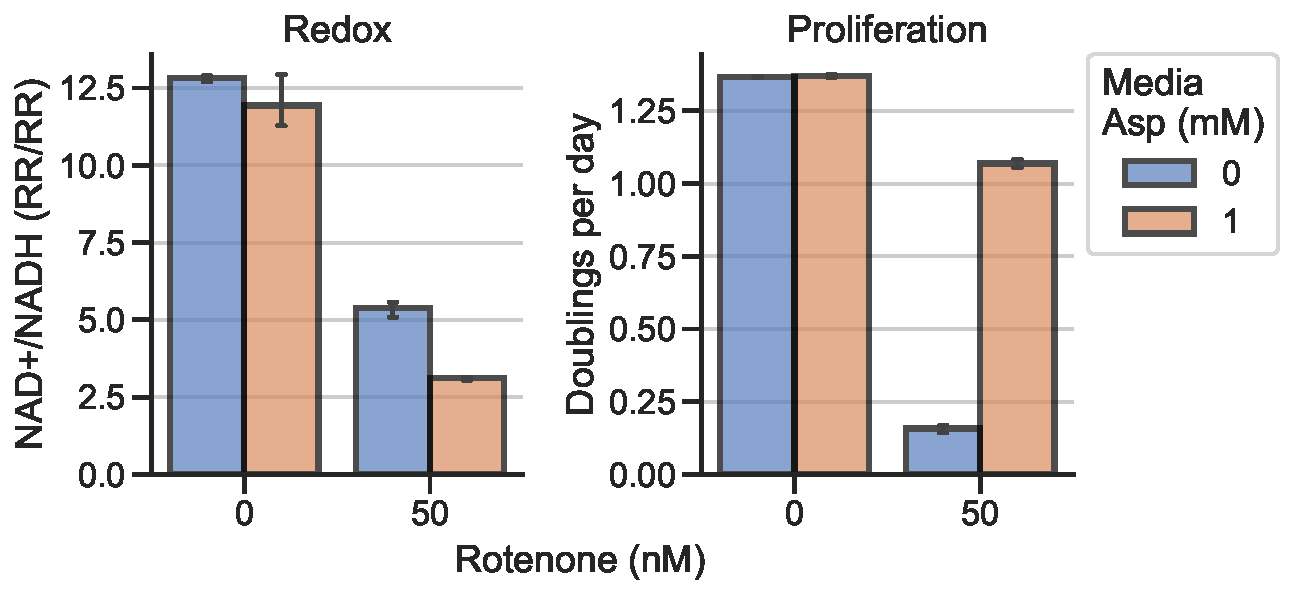
\includegraphics[width=0.70\textwidth]{figures/chap1/redox-prlfr_uncpl.pdf}
    \caption[Aspartate rescues proliferation but not the NAD+/NADH ratio]{
    Aspartate rescues proliferation but not the NAD+/NADH ratio.
    Uncoupling NAD+/NADH and aspartate's effect on proliferation using 143B cells with stable expression of the Glu/Asp transporter SLC1A3, treated with/without 1 mM media aspartate and with/without 50 nM rotenone.
    NAD+/NADH ratio measured using LCMS as a ratio between two internal standard normalized response ratios (RR/RR).
    }
    \label{fig:ch1:redox-prlfr_uncpl}
\end{figure}





